\documentclass[paper=a4, fontsize=11pt]{scrartcl} % A4 paper and 11pt font size

\usepackage[T1]{fontenc} % Use 8-bit encoding that has 256 glyphs
\usepackage[english]{babel} % English language/hyphenation
\usepackage{amsmath,amsfonts,amsthm} % Math packages
\usepackage{graphicx}

\usepackage{lipsum} % Used for inserting dummy 'Lorem ipsum' text into the template

\usepackage{sectsty} % Allows customizing section commands
\allsectionsfont{\centering \normalfont\scshape} % Make all sections centered, the default font and small caps

\usepackage{fancyhdr} % Custom headers and footers
\pagestyle{fancyplain} % Makes all pages in the document conform to the custom headers and footers
\fancyhead{} % No page header - if you want one, create it in the same way as the footers below
\fancyfoot[L]{} % Empty left footer
\fancyfoot[C]{} % Empty center footer
\fancyfoot[R]{\thepage} % Page numbering for right footer
\renewcommand{\headrulewidth}{0pt} % Remove header underlines
\renewcommand{\footrulewidth}{0pt} % Remove footer underlines
\setlength{\headheight}{13.6pt} % Customize the height of the header

\numberwithin{equation}{section} % Number equations within sections (i.e. 1.1, 1.2, 2.1, 2.2 instead of 1, 2, 3, 4)
\numberwithin{figure}{section} % Number figures within sections (i.e. 1.1, 1.2, 2.1, 2.2 instead of 1, 2, 3, 4)
\numberwithin{table}{section} % Number tables within sections (i.e. 1.1, 1.2, 2.1, 2.2 instead of 1, 2, 3, 4)

\setlength\parindent{0pt} % Removes all indentation from paragraphs - comment this line for an assignment with lots of text

%----------------------------------------------------------------------------------------
%	TITLE SECTION
%----------------------------------------------------------------------------------------

\newcommand{\horrule}[1]{\rule{\linewidth}{#1}} % Create horizontal rule command with 1 argument of height

\title{	
	\normalfont \normalsize 
	\textsc{EC500 - Introduction to Learning From Data} \\ [25pt] % Your university, school and/or department name(s)
	\horrule{0.5pt} \\[0.4cm] % Thin top horizontal rule
	\huge Matlab 5 \\ % The assignment title
	\horrule{2pt} \\[0.5cm] % Thick bottom horizontal rule
}

\author{Mikhail Andreev} % Your name

\date{\normalsize\today} % Today's date or a custom date

\begin{document}
	
	\maketitle % Print the title
	

	%----------------------------------------------------------------------------------------
	%	PROBLEM 1
	%----------------------------------------------------------------------------------------
	
	\newpage
	\section{Introduction}
	The problem we are seeking to solve is that of image classification. Given a set of handwritten digits, the goal is to determine the value of an arbitrary digit. I seek to accomplish this through the use of neural networks, specifically using Multi-layer perceptron networks and convolutional networks. Neural networks are well adapted for this level of problem because they can find underlying patterns within the images, contributing to classification. 
	\\\\
	We are interested in this problem because we seek to bridge the gap between human and machine comprehension. For a person, we can look at an image we have never seen before, and in less than a second, we are able to categorize its contents. For a machine without learning techniques, if an image has not been previously defined, it is impossible to categorize. By introducing a learning technique we hope to allow a machine to categorize arbitrary images.
	\newpage
	\section{Literature Review}
	There are many ways to approach the problem of handwritten digit classification.
	\\\\
	In their paper, Fast and Accurate Digit Classification, Subhransu Maji and Jitendra Malik propose using SVMs to classify digits and get a very low error rate of 0.79\%. In his paper, Learning Algorithms for Classification, Yann LeCun and others describe using linear classifiers and K-means as approaches to solving the issue. These approaches got an 8.4\% error and a 2.4\% error respectively.
	\\\\
	In light of the variety of valid approaches, the reason for the usage of neural networks stems back to bridging the gap between human and machine comprehension. Human brains can be thought of as a vast and complicated network of neurons. Each of these neurons takes in a large number of inputs, and depending on the different pathways in the brain, leads to some conclusive thought or action. By modeling this with artificial neural networks, we try to allow machines to understand the world in the same way humans understand it.
	\newpage
	\section{Problem Statement}
	The problem we seek to solve is to classify handwritten images of digits. This gives us the following method for learning. Given a dataset, we first seperate it into a training set and a testing set. We use the training set to build the neural network and optimize the weights between the neurons. Once the set has been trained, we run the testing set through the network and use the output as the classification of the digits. Two networks are used and analyzed for this problem. The first approach is the Multi-Layer Perceptron(MLP). This is a basic model for the neural network approach. The second network is the Convolutional Network. While this network still holds with the basic framework of MLP, it changes it to use convolution and pooling to classify patterns. Although these networks are used for classification, the actual method of this classification is through regression. The image pixels are processed as real values and the end result is also a real value, which is then interpreted as a label.
	\\\\
	\subsection{Dataset}
	The dataset that will be used for this problem is the MNIST dataset of handwritten digits. This consists of 10 files each containing 1000 images. Each digit is a handwritten number, corresponding to the number of the file. For example, if the file is named data0, it contains 1000 images of handwritten 0s. Each of the digits is formed by a 28x28 matrix of greyscale values ranging from 0 to 255. When input into the code for Multi-Layer Perceptron, the images are modified for more ease of processing. This modification consists of changing any non-zero value to a 1. The resulting image consists entirely of 0s and 1s.  
	\\\\
	\subsection{Neuron}
	Before we can analyze the neural networks, we must first discuss how a single neuron functions. The below figure illustrates the basic structure of a neuron:
	\\\\
	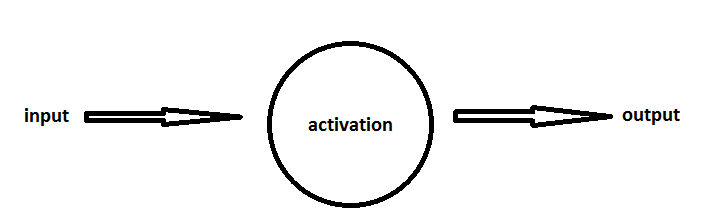
\includegraphics[scale=0.7]{neuron}
	\\\\
	The input that goes into the neuron is passed to its activation function. This activation function can produce non-linear behavior. Typically, the activation function used varies based on which layer the neuron is in. Some typical activation functions include:\\\\
	$$f_{LINEAR}(z) = z$$\\\\
	$$f_{SIGMOID}(z) = \frac{1}{1-e^{-z}}$$\\\\
	$$f_{TANH}(z) = \frac{e^z-e^{-z}}{e^z+e^{-z}}$$\\\\
	The sigmoid and the hyperbolic functions have a range of 0 to 1 and -1 to 1 respectively creating non-linear output. Generally these are used in the hidden layers of an MLP while the linear activation is used for the input and output layers.
	\\\\
	\subsection{Multi-Layer Perceptron}
	By creating a network of the neurons presented above we can achieve non-linear modeling of an algorithm. By creating multiple layers of neurons and connecting them, we create a Multi-Layer Perceptron network.
	\\\\
	\hspace*{-.1cm}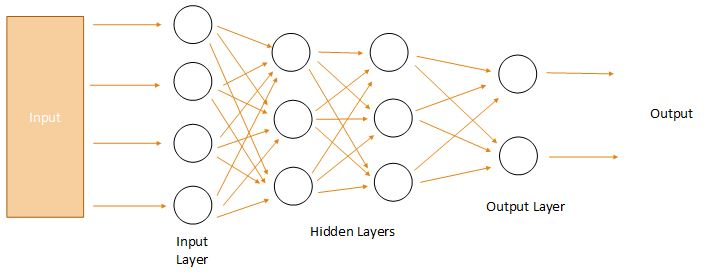
\includegraphics[scale=0.9]{mlp}
	\\\\
	The basic structure of a MLP is shown above. The input example gets passed through to the input layer. Usually, each feature of the example is passed to a seperate input neuron. After the input layer there are one or more hidden layeres with non-linear activation functions. The input to each of the hidden layer neurons is a weighted sum of the values of the previous layer. This weighted sum is then passed into activation function to generate the value of the current network. Using this mechanism, the values are passed into the output layer, whose final response forms the response of the network. In this model, all neurons in one layer are connected to all neurons in the following layer. 
	\\\\
	The mechanism of passing values through the network is called the feed-forward stage. It is used to generate the output of the network and the classification of the image. The value at each neuron through the feed-forward mechanism can be written as:
	\\\\
	$$y^{(l)}_j = f( \sum_{i} y^{(l-1)}_i w_{ji})$$
	\\\\
	Here, $y^{(l)}_j$ is the value of the j-th neuron on l-th layer. $y^{(l-1)}_i$ is the value of the i-th neuron on the previous layer (l-1). $w_{ji}$ is the weight of the connection between the neurons i and j. Finally, $f()$ is the activation function of j-th neuron. This equation means that you take the value of all the neurons in the previous layer, multiply it by the weight of the connection between each neuron, and sum the result. After that pass the result into the activation function of the j-th neuron, and set the value of that neuron to the output of the activation function.
	\\\\
	After we have obtained the output value of the network, the next step in training is to calculate the error between the obtained value and the desired value:
	\\\\
	$$E(w, D) = \frac{1}{2}\sum_i^{outputs}||y_{computed}^{(i)} - y_{actual}^{(i)}||^2$$
	\\\\
	With this error, we calculate the derivatives of the neuron values with respect to the neuron weights, and use this to update the weights. This technique is called gradient descent. By first calulating the change in weight at the output neurons, then using the derivative values to calculate the change in weight in the previous layer, we propogate backwards through the network. This gives us the mechanism of back-propogation.
	\\\\
	The derivative or delta values calculated are different if the current node is an output node or a hidden node. The reason for this is because the output nodes can simply use the desired output to calculate the necessary weight change. Meanwhile the hidden layers must use the calculated values of the layer ahead of them. The delta for the output layer can be written as this:
	\\\\
	$$\Delta_i^{(L)} = (y_{computed}^{(i)} - y_{actual}^{(i)})f'(y^{(i)})$$
	\\\\
	Using these values for the calculated for output node deltas, we can then calculate the delta values of the hidden nodes with the following equation:
	\\\\
	$$\Delta_i^{(l)} =  \sum^{l+1}_k \Delta_k^{(l+1)}w_{ki}^{(l+1)}f'(y_i^{(l)})$$
	\\\\
	After we have calculated all the delta values for each node, we update the weights using the following formula:
	\\\\
	$$\Delta w_{ji}^{(l)} = w_{ji}^{(l)} + \eta\Delta_j^{(l)}y_i^{(l-1)}$$
	\\\\
	Here $\eta$ is the learning rate of our neural network. The higher the learning rate the more quickly the weights change. However, if the learning rate is too high, the weights will diverge, and increase to infinity. 
	\\\\
	By repetedly updating the weights our network eventually reaches a point where it is able to predict the labels of a testing sample. There are two methods of training the neural network based on when the weights are updated. The first method is to update by pattern, updating the weights after each example. This training method is fairly fast since you only have to run through the examples once. The second method takes longer but generally produces better results. This is known as update by epoch. In this method, you run all the examples through and calculate the overall weight change. After applying the weight change, you run the examples again. By doing this repetedly, we achive a convergence of the weights.
	\subsection{Convolutional Network}
	The convolutional network follows the same steps as the MLP network, although with different structure. This difference in structure allows the convolutional network to become a better classifier. In the particular case of this problem, the convolutional network takes advantage of the structure of an image. The MLP treats all pixels as being right next to each other since all inputs are passed to all hidden nodes. However, the convolutional network is different because it takes into account pixel proximity. 
	\\\\
	The convolutional network has 3 main differences from the MLP. The first of these is known as local receptive fields. This means that instead of the first hidden layer nodes all getting each of the input values, they get a small set of the input values. For example, a hidden layer node may take a 5x5 block from the input data. All the inputs to a given node of the hidden layer are weighted and biased in the same manner, forming the second difference between the two methods. The end result is a feature map of that subset of the input image. The equation demonstrating this can be written as:
	\\\\
	$$y_{jk} = f(\sum_{l}\sum_{m}w_{lm}a_{j+l, k+m})$$
	\\\\
	The feature map created by these operations result in the detection of some part of an image such as an edge or a curve. This allows that feature to be detected anywhere it is found in an image. This breaks the input image down into a set of more basic features, learning internal image patterns as opposed to some general overall shape. Since multiple features are present in an image, multiple receptive fields or feature maps are created at the same time.
	\\\\
	The third difference between MLP and convolutional neural networks is the introduction of the pooling layer. The pooling layer aggregates the different values in a feature map and combines them to simplify the output. This allows less relevant features to not have a negative impact on the prediction. After the pooling layer, the results are sent to the output layer where they lead to classification. The diagram below demonstrates the structure of the convolutional network. 
	\\\\
	\hspace*{-.1cm}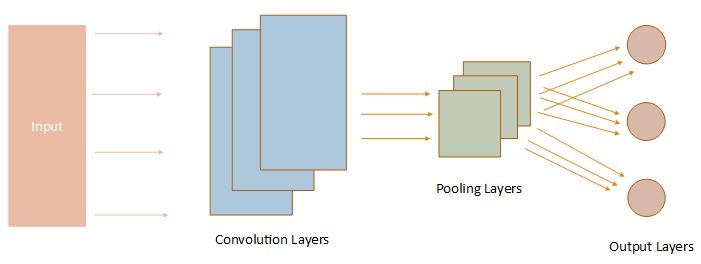
\includegraphics[scale=0.9]{conv}

	\newpage
	\section{Implementation}
	The MLP network was implemented using MATLAB. The program flow was to load all the image data into matrices as the examples. After this the network was created. The input layer was set to 784 neurons, matching the number of pixels in the image. From there, the number of layers and the number of neurons in each layer was varied to determine optimal structure. The weights between the layers and the values at each neuron were held in a set of matrices. By using matrices to store these values, many of the calculations described above were done in parallel multiplication. This allowed for a very fast implementation. The number of output neurons used was determined by the number of categories used in classification. The weights were randomly assigned between the values of -.5 and .5.
	\\\\
	To calculate the convolutional network, code provided by Michael Nielsen (https://github.com/mnielsen/neural-networks-and-deep-learning) was used. This code used the Theano python library to create and test the convolutional network. I used this code to run some tests for different neuron configurations.
	
	\newpage
	\section{Experimental Results}
	The overall results found during testing is displayed here. This was found by testing the network repetedly with different parameters. The best general results are shown here with the parameters displayed. The results in this chart are for 3 types of digits with 300 training images in each category.
	\\\\
	\hspace*{-.1cm}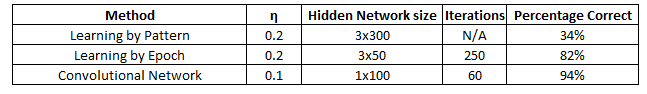
\includegraphics[scale=0.9]{overall_results}
	\\\\
	As can be seen from the chart, of the MLP networks, learning by epoch produced much better results, indicating better learning in the network. The performance of the convolutional network was much higher than either of two MLP networks, indicating the superior pattern learning.
	\\\\
	A demonstration of the success of different parameters can be seen here for the MLP learning by epoch network.
	\\\\
	\hspace*{-.1cm}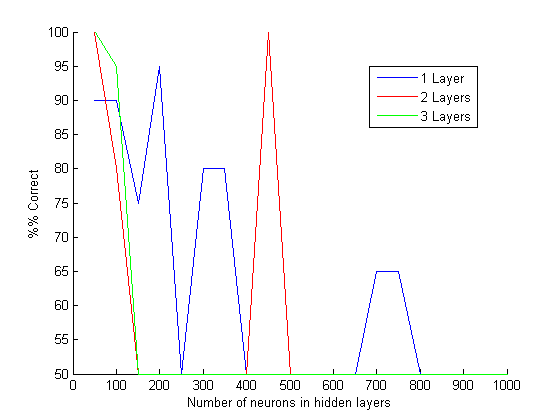
\includegraphics[scale=0.9]{num_neurons_for_learning}
	\\\\
	This graph shows the percent correct rate versus the number of neurons per layer. The three different color lines indicate the number of layers used. As can be seen, better results are generally found for fewer neurons, indicating that too many neurons leads to overfitting for the test examples.
	\newpage
	\section{Conclusions}
	Neural networks are a powerful tool in the field of classfication. By combining large numbers of neurons and layers, one can make very complicated learning structures. The parameters of neural network need to be well tested to find the optimal arrangement and get the best results. Different learning strategies and activation functions will get better results in some scenarios, and worse in others depnding on the distribution of the data.
	\\\\
	To further improve the results, more testing of the parameters and functions is required. New learning methods can be introduced such as momentum or adaptive learning rates. Once high results can be obtained for the current data set, a more complicated dataset can be used to see how the network will perform on more difficult images. 
	\\\\
	\newpage
	\section{Description of Individual Effort}
	The project had only one member.
	\newpage
	\section{References}
	Machine Learning: Multi Layer Perceptrons - Prof. Dr. Martin Riedmiller
	\\\\
	Deep Learning - Michael Nielsen, (http://neuralnetworksanddeeplearning.com/chap6.html)
	\\\\
	Convolutional Neural Network Committees For Handwritten Character Classification - Dan Claudiu Cires, Ueli Meier, Luca Maria Gambardella, Jurgen Schmidhuber
	\\\\
	Fast and Accurate Digit Classification - Subhransu Maji and Jitendra Malik, (http://www.eecs.berkeley.edu/Pubs/TechRpts/2009/EECS-2009-159.html)
	\\\\
	Learning Algorithms for Classification - Yann LeCun, (http://yann.lecun.com/exdb/publis/pdf/lecun-95a.pdf)
	\newpage
	\section{Appendix}
	The code is included in the zipped submission.
	
	
\end{document}